\section{Functional Specification}

This section provides a comprehensive overview of the system's functionality. It includes a use case diagram illustrating the system's interactions and a detailed textual description of each use case.

\subsection{Use Case Diagram}

Figure \ref{fig:Sprint 3 Use Case Diagram} offers us an overview by presenting a visual description of the functional
behaviour of our tool during the third sprint. This diagram sums up the interactions among the actors and the
diverse use cases within the system.

\begin{figure}[ht]
	\centering
	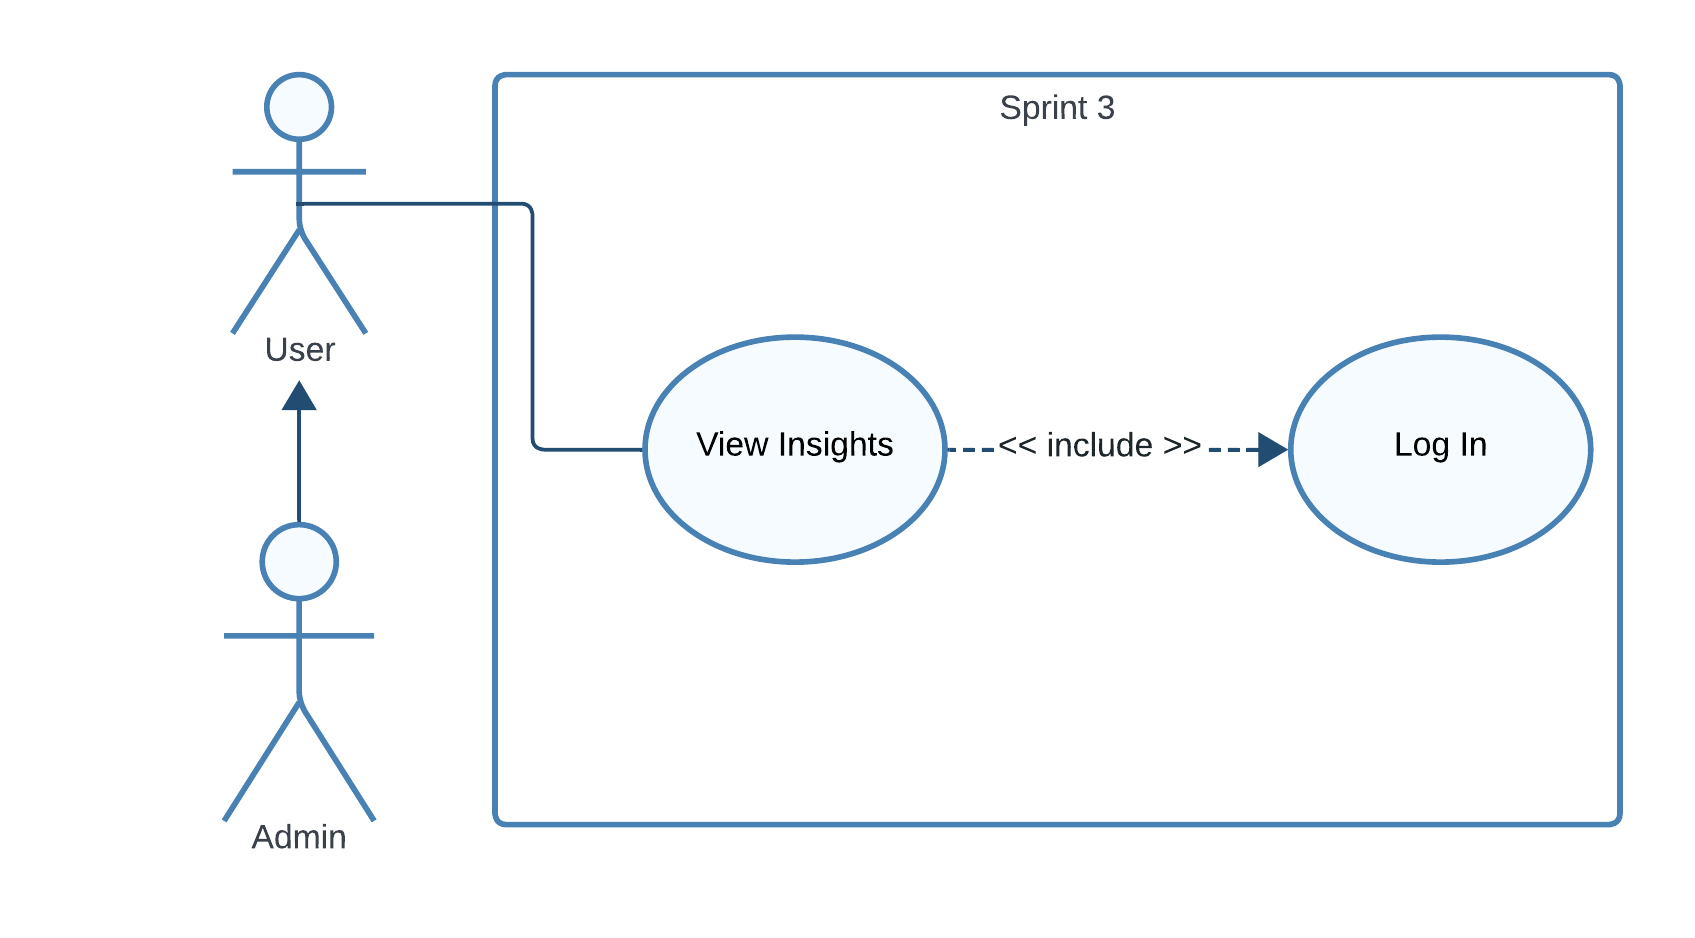
\includegraphics[width=\linewidth]{Images/Sprint3/use case diag.png}
	\caption{Sprint 3 Use Case Diagram}
	\label{fig:Sprint 3 Use Case Diagram}
\end{figure}

\subsection{Textual Description of Use Cases}

The following tables provide a detailed description of the use cases. This includes the actor, the goal of the use case, the preconditions, the basic flow, the alternative flows, and the postconditions.

\subsubsection{Use Case 1 View Insights}

Table \ref{tab:Use Case 1 View Insights} presents a textual description of a use case: View Insights.

\clearpage

\begin{table}[ht]
	\centering
	\begin{tabularx}{\textwidth}{|l|X|}
		\hline
		\textbf{Actor}             & User, Admin                                                                                         \\
		\hline
		\textbf{Goal}              & To view insights of a published campaign                                                            \\
		\hline
		\textbf{Preconditions}     & A campaign has been published and tracking data is available                                        \\
		\hline
		\textbf{Basic Flow}        & 1. The user selects a published campaign from the list of campaigns.                                \\
		                           & 2. The system retrieves and displays the insights details for the selected campaign.                \\
		\hline
		\textbf{Alternative Flows} & If no tracking data is available, the system informs the user and prompts them to check back later. \\
		\hline
		\textbf{Postconditions}    & The user has viewed the insights for the selected campaign.                                         \\
		\hline
	\end{tabularx}
	\caption{Use Case 1: View Insights}
	\label{tab:Use Case 1 View Insights}
\end{table}